\documentclass[11pt,a4paper]{article}
\usepackage[T1]{fontenc}
\usepackage[utf8]{inputenc}
\usepackage[sc]{mathpazo}
\linespread{1.04}
\usepackage[scaled=0.86]{helvet}
\usepackage[margin=1in]{geometry}
\usepackage{amsmath,amssymb,amsthm,mathtools}
\usepackage{booktabs}
\usepackage{array}
\usepackage{tabularx}
\usepackage{float}
\usepackage[hidelinks]{hyperref}
\usepackage[nameinlink,noabbrev]{cleveref}
\usepackage{microtype}
\usepackage{enumitem}
\usepackage{siunitx}
\usepackage{xcolor}
\usepackage{caption}
\usepackage{tcolorbox}
\tcbuselibrary{skins,breakable}
\usepackage{thmtools}
\usepackage{tikz}
\usetikzlibrary{arrows.meta,positioning,calc,fit,backgrounds,matrix,decorations.pathmorphing}
\usepackage{pgfplots}
\pgfplotsset{compat=1.18}
\usepackage{longtable}
\usepackage{multirow}
\usepackage{makecell}
\usepackage{bm}
\usepackage{csquotes}
\usepackage{fancyhdr}
\usepackage{titlesec}

% ── Color palette ──
\definecolor{tfptblue}{RGB}{35,60,120}
\definecolor{tfptorange}{RGB}{190,100,20}
\definecolor{tfptgreen}{RGB}{40,110,60}
\definecolor{tfptgray}{RGB}{90,90,95}

\hypersetup{
    colorlinks=true,
    linkcolor=tfptblue!80!black,
    citecolor=tfptblue!70!black,
    urlcolor=tfptblue!60!black,
}

% ── Caption styling ──
\captionsetup{
    font={small,sf},
    labelfont={bf,color=tfptgray},
    labelsep=period,
    margin=1.5em,
    skip=6pt,
}

% ── Section heading styling ──
\titleformat{\section}
    {\Large\bfseries\color{tfptblue}}{\thesection}{0.8em}{}
\titleformat{\subsection}
    {\large\bfseries\color{tfptblue!85!black}}{\thesubsection}{0.7em}{}
\titleformat{\subsubsection}
    {\normalsize\bfseries\color{tfptblue!70!black}}{\thesubsubsection}{0.6em}{}
\titlespacing*{\section}{0pt}{1.8ex plus 0.6ex minus 0.3ex}{0.9ex plus 0.2ex}
\titlespacing*{\subsection}{0pt}{1.4ex plus 0.4ex minus 0.2ex}{0.6ex plus 0.1ex}

% ── Running headers ──
\pagestyle{fancy}
\setlength{\headheight}{22pt}
\fancyhf{}
\fancyhead[L]{\small\itshape\color{tfptgray} TFPT 4.5: Boundary Polarization and Closed-Branch Dynamics}
\fancyhead[R]{\small\color{tfptgray}\thepage}
\renewcommand{\headrulewidth}{0.4pt}
\renewcommand{\headrule}{\hbox to\headwidth{\color{tfptblue!30}\leaders\hrule height \headrulewidth\hfill}}
\fancypagestyle{plain}{\fancyhf{}\fancyfoot[C]{\small\color{tfptgray}\thepage}\renewcommand{\headrulewidth}{0pt}}

% ── tcolorbox global defaults ──
\tcbset{
    enhanced,
    boxrule=0.6pt,
    arc=2.5pt,
    left=6pt, right=6pt, top=5pt, bottom=5pt,
    fonttitle=\bfseries\sffamily\small,
    coltitle=white,
    toptitle=2pt, bottomtitle=2pt,
    shadow={0.8mm}{-0.6mm}{0mm}{black!12},
}

\sisetup{
    detect-all,
    round-mode = none,
    exponent-mode = input,
    exponent-product = \times,
    group-separator = {\,},
    group-minimum-digits = 4
}

\newtheorem{theorem}{Theorem}[section]
\newtheorem{corollary}[theorem]{Corollary}
\newtheorem{lemma}[theorem]{Lemma}
\theoremstyle{definition}
\newtheorem{definition}[theorem]{Definition}
\newtheorem{conjecture}[theorem]{Conjecture}
\newtheorem{proposition}[theorem]{Proposition}
\newtheorem{assumption}[theorem]{Assumption}
\newtheorem{axiom}[theorem]{Axiom}
\newtheorem{principle}[theorem]{Principle}
\newtheorem{construction}[theorem]{Construction}
\newtheorem{claim}[theorem]{Claim}
\newtheorem{appendixstep}[theorem]{Appendix Step}
\theoremstyle{remark}
\newtheorem*{remark}{Remark}

\crefformat{thmt@dummyctr}{Remark}
\Crefformat{thmt@dummyctr}{Remark}
\crefname{thmt@dummyctr}{remark}{remarks}
\Crefname{thmt@dummyctr}{Remark}{Remarks}
\crefname{conjecture}{conjecture}{conjectures}
\Crefname{conjecture}{Conjecture}{Conjectures}
\crefname{definition}{definition}{definitions}
\Crefname{definition}{Definition}{Definitions}

\makeatletter
\def\theHtheorem{\thesection.\thetheorem}
\def\theHcorollary{\theHtheorem}
\def\theHlemma{\theHtheorem}
\def\theHdefinition{\theHtheorem}
\def\theHconjecture{\theHtheorem}
\def\theHproposition{\theHtheorem}
\def\theHassumption{\theHtheorem}
\def\theHprinciple{\theHtheorem}
\def\theHconstruction{\theHtheorem}
\def\theHclaim{\theHtheorem}
\def\theHappendixstep{\theHtheorem}
\makeatother

\DeclareMathOperator{\tr}{Tr}
\DeclareMathOperator{\rank}{rank}
\DeclareMathOperator{\SF}{SF}
\DeclareMathOperator{\Ind}{Ind}
\DeclareMathOperator{\argmin}{arg\,min}

\newcolumntype{Y}{>{\raggedright\arraybackslash}X}

\newcommand{\Seam}{\Sigma}
\newcommand{\inv}{\iota}
\newcommand{\taudbl}{\tau_{\mathrm{dbl}}}
\newcommand{\iC}{\iota_{\mathrm C}}
\newcommand{\epscar}{\varepsilon_{\mathrm{car}}}
\newcommand{\Xbulk}{X_{\mathrm{bulk}}}
\newcommand{\Mpl}{\bar M_{\mathrm{Pl}}}
\newcommand{\Mplunred}{M_{\mathrm{Pl}}}
\newcommand{\cthree}{c_3}
\newcommand{\atheta}{a_\theta}
\newcommand{\phibase}{\varphi_{\mathrm{base}}}
\newcommand{\phiz}{\varphi_0^{\mathrm{ret}}}
\newcommand{\phiseam}{\varphi_{\Sigma}}
\newcommand{\deltatop}{\delta_{\mathrm{top}}}
\newcommand{\omegaCCEW}{\omega_{\mathrm{CC}}^{(2)}}
\newcommand{\bone}{b_1}
\newcommand{\SM}{\mathrm{SM}}
\newcommand{\QCD}{\mathrm{QCD}}
\newcommand{\Oadm}{\Omega_{\mathrm{adm}}}
\newcommand{\Cmin}{\mathcal C_{\min}}
\newcommand{\Ageom}{\mathcal A_{\mathrm{geom}}}
\newcommand{\Atrans}{\mathcal A_{\mathrm{trans}}}
\newcommand{\Arec}{\mathcal A_{\mathrm{rec}}}
\newcommand{\Aobs}{\mathcal A_{\mathrm{obs}}}
\newcommand{\Asing}{\mathcal A_{\mathrm{sing}}}
\newcommand{\Vadm}{\mathcal V_{\mathrm{adm}}}
\newcommand{\Hrel}{\mathcal H_{\mathrm{rel}}}
\newcommand{\Hhad}{\mathcal H_{\mathrm{had}}}
\newcommand{\Hhub}{H_{\mathrm{hub}}}
\newcommand{\Htot}{\mathcal H_{\mathrm{tot}}}
\newcommand{\Gammaeff}{\Gamma_{\mathrm{eff}}}
\newcommand{\lambdaY}{\lambda_Y}
\newcommand{\Pred}{\operatorname{Pred}}
\newcommand{\gcar}{g_{\mathrm{car}}}
\newcommand{\Hint}{\mathcal H_{\mathrm{int}}}
\newcommand{\Kadm}{K_{\mathrm{adm}}}
\newcommand{\Tmin}{\mathfrak T_{\mathrm{min}}}
\newcommand{\Tbound}{\mathfrak T_{\partial}^{\min}}
\newcommand{\Tprim}{\mathfrak T_{\mathrm{prim}}}
\newcommand{\chiseed}{\chi_{\mathrm{seed}}}
\newcommand{\chigeo}{\chi_{\mathrm{geo}}}
\newcommand{\chigeozero}{\chi_{\mathrm{geo},0}}
\newcommand{\APSdom}{\mathrm{APS}_{\mathrm{dom}}}
\newcommand{\APSfam}{\mathrm{APS}_{\mathrm{fam}}}
\newcommand{\vgeo}{v_{\mathrm{geo}}}
\newcommand{\vewref}{v_{\mathrm{EW}}^{\mathrm{ref}}}
\newcommand{\Dstart}{D_{\mathrm{start}}}
\newcommand{\Tcore}{\mathfrak T_{\mathrm{core}}}
\newcommand{\Tbridge}{\mathfrak T_{\mathrm{bridge}}}
\newcommand{\Tker}{\mathfrak T_{\mathrm{ker}}}
\newcommand{\Tcomp}{\mathfrak T_{\mathrm{comp}}}
\newcommand{\Padm}{P_{\mathrm{adm}}}
\newcommand{\Pprim}{P_{\mathrm{prim}}}
\newcommand{\Tpre}{\mathfrak T_{\mathrm{pre}}}
\newcommand{\Tstar}{\mathfrak T_{\star}}
\newcommand{\APSdomprov}{\mathrm{APS}_{\mathrm{dom}}^{\mathrm{prov}}}
\newcommand{\sigmaQCD}{\sigma_{\mathrm{QCD}}}
\newcommand{\Cseam}{\mathcal C_{\Sigma}}
\newcommand{\Ccyc}{\mathfrak C_{\Sigma}}
\newcommand{\Ffals}{\mathsf F_{\mathrm{fals}}}
\newcommand{\Rcmp}{\mathcal R_{\mathrm{cmp}}}
\newcommand{\wspin}{\varpi_{\mathrm{spin}}}
\newcommand{\PhysAdmOne}{\widehat{\mathrm{PhysAdm}}_1}
\newcommand{\ObsAdm}{\mathbf{Obs}_{\mathrm{adm}}}
\newcommand{\GrenTFPT}{\Gamma_{\mathrm{TFPT}}^{\mathrm{ren}}}
\newcommand{\OphysTFPT}{\mathbf O_{\mathrm{phys}}^{\mathrm{TFPT}}}
\newcommand{\OschemeTFPT}{\mathbf O_{\mathrm{scheme}}^{\mathrm{TFPT}}}
\newcommand{\SchGrp}{\mathbf{Sch}}
\newcommand{\Runiv}{\mathfrak R}
\newcommand{\Mop}{\mathfrak M}
\newcommand{\Mphys}{\mathfrak M_{\mathrm{phys}}}
\newcommand{\Mscheme}{\mathfrak M_{\mathrm{scheme}}}
\newcommand{\Rren}{\mathfrak R_{\mathrm{ren}}}
\newcommand{\Bind}{\mathcal B_{\mathrm{ind}}}
\newcommand{\Clrig}{\mathfrak{Cl}}
\newcommand{\Runivrig}{\overline{\Runiv}}
\newcommand{\Seedop}{\mathbf{Seed}^{\mathrm{op}}}
\newcommand{\Cseed}{\mathfrak C_{\mathrm{seed}}}
\newcommand{\triv}{\textup{triv}}
\newcommand{\rankess}{\rank_{\textup{ess}}}
\newcommand{\red}{\textup{red}}


% -- TFPT 4.5 split helpers --
\newcommand{\sourceDraft}{\texttt{../tfpt-42.tex}}
\newcommand{\paperstatus}{Draft split from \sourceDraft; theorem wording still inherits the status discipline of the source manuscript.}

\newenvironment{tfptfrontbox}
{\begin{tcolorbox}[colback=tfptblue!2, colframe=tfptblue!45, breakable,
    title={Scope box: inputs, contribution, non-claims, audit surface}, colbacktitle=tfptblue!65]}
{\end{tcolorbox}}

\newenvironment{tfptwarningbox}
{\begin{tcolorbox}[colback=tfptorange!4, colframe=tfptorange!55, breakable,
    title={Editorial guardrail}, colbacktitle=tfptorange!75]}
{\end{tcolorbox}}

\newenvironment{tfptsourcebox}
{\begin{tcolorbox}[colback=tfptgreen!3, colframe=tfptgreen!50, breakable,
    title={Source extraction map}, colbacktitle=tfptgreen!65]}
{\end{tcolorbox}}

\newcommand{\TFPTxref}[1]{\textup{[TFPT cross-reference: \texttt{\detokenize{#1}}]}}
\newcommand{\TFPTeqref}[1]{\textup{[TFPT equation: \texttt{\detokenize{#1}}]}}

\newenvironment{tfptclaimcontract}
{\begin{tcolorbox}[colback=tfptblue!2, colframe=tfptblue!50, breakable,
    title={Claim contract}, colbacktitle=tfptblue!70]\small}
{\end{tcolorbox}}

\newenvironment{tfptexports}
{\begin{tcolorbox}[colback=tfptgreen!3, colframe=tfptgreen!50, breakable,
    title={Exported objects}, colbacktitle=tfptgreen!65]}
{\end{tcolorbox}}



\title{\color{tfptblue}\textbf{Boundary Polarization and the Primitive Kernel of TFPT}}
\author{Stefan Hamann \and Alessandro Rizzo}
\date{{\normalsize\color{tfptgray}\sffamily Paper 1 of the TFPT 4.5 series -- \today}}

\begin{document}
\maketitle

\begin{abstract}
This paper isolates the primitive boundary kernel. Starting from the minimal operational seed and
the one-sided boundary datum, it reconstructs the exact double, the deck involution, the Calderon
polarization, the primitive admissibility complex, the primitive seam generator, the winding
normalization $[u_\Sigma]=1$, and the normalization $\cthree=1/(8\pi)$. No Standard-Model,
phenomenological, gravitational, cosmological, or E8 claim is made in this paper.
\end{abstract}

\begin{tfptfrontbox}
\textbf{Inputs from previous papers.} Only the orientation map of Paper 0, if read first.

\textbf{New theorem contribution.} The primitive kernel
\[
\Tker^\partial=(\mathcal A,\mathcal H,D,J,\Gamma,\taudbl,\iC,\Pprim,[u_\Sigma],\cthree)
\]
is reconstructed from the one-sided boundary datum rather than inserted later.

\textbf{Not claimed here.} No carrier $3+2$ theorem, no Standard-Model gauge group, no $\alpha$,
no flavor, no gravity, no cosmology, and no E8 scale grammar.

\textbf{Falsification or audit surface.} The paper fails if the one-sided datum does not determine
the doubled datum, the Calderon polarization, the primitive Hodge selector, or the normalization of
the primitive seam class.
\end{tfptfrontbox}


\begin{tfptclaimcontract}
\textbf{Claim.} $\mathfrak S_{\min}\Rightarrow\mathcal B_{\min}\Rightarrow\Tbound\Rightarrow(\taudbl,\iC,\Pprim,[u_\Sigma],\cthree)$.\par
\textbf{Inputs.} One-sided admissible boundary datum and stated boundary-elliptic regularity.\par
\textbf{First assumptions.} Product collar, ellipticity, self-adjoint boundary realization, Calderon uniqueness, orientation normalization.\par
\textbf{Proof status.} Core theorem target for the primitive kernel.\par
\textbf{Kill condition.} Failure of the boundary datum to determine $P_C$, $\iC$, $\taudbl$, $\Pprim$, $[u_\Sigma]$, or $\cthree$.\par
\end{tfptclaimcontract}

\tableofcontents

\section{Claim Map}

The paper proves the first load-bearing arrow of the TFPT series:
\[
\mathfrak S_{\min}
\Rightarrow
\mathcal B_{\min}
\Rightarrow
\Tbound
\Rightarrow
(\taudbl,\iC,\Pprim,[u_\Sigma],\cthree).
\]
All later discrete, physical, and numerical structures are treated as unavailable here. The purpose
is to make the boundary primitive kernel auditable on its own.

\begin{tfptwarningbox}
Minimality is used only as a presentation-invariant defect filtration on essentialized admissible
bordisms. It is not a preference order over desired physics. In particular, the corner count and
the later $3+2$ carrier ranks are not free minimization coordinates in this paper.
\end{tfptwarningbox}

\section{One-Sided Boundary Datum}

The starting object is
\[
\Tbound=(\mathcal A_+,\mathcal H_+,D_+,J,\Gamma,B_\Sigma).
\]
The paper should keep only the source manuscript material needed to explain one-sided admissible
data, induced boundary spectral data, and the passage to a doubled closed datum. The proof burden is
that the primitive boundary structure is not chosen by hand.

\section{Exact Double and Deck Involution}

The exact double reconstructs
\[
\Tmin^{\mathrm{cl}}=(\mathcal A,\mathcal H,D,J,\Gamma,\taudbl,\iC)
\]
with $\taudbl$ as deck involution and $\iC$ as the involution induced by the Calderon polarization.
This section carries the analytic interface to Calderon projectors and the primitive relative
spectral dynamics from the source draft.

\section{Primitive Admissibility Complex}

The primitive selector is introduced before any color, determinant, family, or QFT sector:
\[
\Pprim=\Pi_{\ker\Delta_{\mathrm{prim}}}.
\]
The section should include the primitive admissibility differential, the primitive Hodge form, and
the selector upgrade logic only as far as it is needed to prove that a later full selector can
factor through $\Pprim$.

\section{Primitive Seam Generator}

The primitive seam generator records the two normalizations that are allowed to survive this paper:
\[
[u_\Sigma]=1,
\qquad
\cthree=\frac{1}{8\pi}.
\]
The winding class is a primitive boundary output. It is not yet a family-counting or flavor
transport input; those interpretations are postponed to Papers 2 and 3.

\section{Boundary Primitive Kernel}

\begin{theorem}[Primitive boundary kernel]
Under the one-sided boundary hypotheses and the primitive admissibility assumptions stated above,
the minimal boundary datum canonically determines
\[
\Tker^\partial
=
(\mathcal A,\mathcal H,D,J,\Gamma,\taudbl,\iC,\Pprim,[u_\Sigma],\cthree).
\]
\end{theorem}

\begin{proof}[Proof structure]
The proof follows the source draft in four steps: operational seed to boundary datum; boundary
datum to exact double; Calderon polarization to $\iC$ and $\Pprim$; primitive seam normalization to
$[u_\Sigma]=1$ and $\cthree=1/(8\pi)$. The paper must keep the representation-theoretic carrier
and all observable readouts out of the argument.
\end{proof}

\section{Audit Protocol}

\begin{center}
\begin{tabularx}{\textwidth}{@{}p{0.24\textwidth}Y@{}}
\toprule
\textbf{Audit item} & \textbf{Question} \\
\midrule
One-sided datum & Is every primitive object reconstructed from $\Tbound$ or from standard boundary spectral data? \\
Calderon interface & Are regularity and projection hypotheses explicit? \\
Primitive selector & Does $\Pprim$ precede the later singlet and determinant projections? \\
Winding class & Is $[u_\Sigma]=1$ fixed before any family or flavor interpretation? \\
Normalization & Is $\cthree=1/(8\pi)$ derived without empirical input? \\
\bottomrule
\end{tabularx}
\end{center}

\clearpage
\section{Main Technical Development}

This section contains the main technical development assigned to this paper by the TFPT 4.5 clean split. Cross-paper background is referenced through dependency and scope boxes; extended backend material is kept in the Technical Companion.

% Auto-extracted from ../tfpt-42.tex for the TFPT 4.5 clean split.
% Source body assigned by the TFPT 4.5 clean split.

% ---- Primitive core and primitive relative spectral dynamics: source lines 849-1305 ----
\section{Primitive core and hard carrier kernel}

\subsection{Primitive core and conventions}

We use natural units $c=\hbar=1$. Relative operators are formulated in Euclidean signature and compared through a declared Wick-rotation bridge when Lorentzian language is needed. Higgs fields are denoted by $\Phi$, Hamiltonians by $\mathcal H$, and the cosmological Hubble rate by $\Hhub(t)$; this avoids overloading the letter $H$. Newton's constant is always $G_N$, while $G_{\mathrm{car}}$ is reserved for the internal carrier stabilizer. The seam is denoted by $\Seam$, geometric reflection by $\taudbl$, boundary polarization by $\iC$, carrier polarization by $\epscar$, and word parity by $\varepsilon(w)$.

Here $S\to \widetilde M$ denotes the spinor bundle on the oriented double cover, and by the same symbol we denote its restriction to
\[
\Xbulk=\widetilde M\setminus\Seam.
\]

When color-center notation is needed later, we use multiplicative notation
\[
z(w)\in\{1,\omega,\omega^2\},
\qquad
\omega=e^{2\pi i/3}.
\]
Thus center neutrality means $z(w)=1$.

\[
\Tcore^{\mathrm{kin}}
:=
\bigl(
\widetilde M\to M,\ \Seam,\ \taudbl,\ \iC,\ D_{\mathrm{ref}},\ D_{\mathrm{rel}},\ \chiseed
\bigr).
\]
When a chosen almost-commutative factorization
$\mathcal H\cong L^2(\widetilde M,S)\otimes\Hint$ is used, $S$ and $\Hint$ refer to that
choice and are not part of the kinematic core datum.
Here \enquote{relative} always means comparison with a declared reference operator or
reference-subtracted action. The canonical admissibility complex is introduced immediately below,
while any Bernstein or other spectral test profile is treated only as an analytic realization
choice rather than as part of the boundary datum. The technical tables for relative objects,
layered closure/benchmark data, and the constants atlas are collected in
Appendix~\ref{app:tech} and Appendix~\TFPTxref{app:constants}; they are kept out of the early
main-text flow so that the carrier kernel appears before the technical bookkeeping apparatus.

\begin{remark}[Boundary datum versus derived closed structure]
The primitive ontology now stops one step earlier. The one-sided boundary datum $\Tbound$
contains only one-sided operator data together with the self-adjoint boundary operator
$B_\Sigma$. Its Calder\'on projector defines the polarization
\[
\iC:=2P_C-1.
\]
From that boundary polarization and the exact double one reconstructs the deck involution
$\taudbl$, the physical quotient $M=\widetilde M/\taudbl$, the seam
$\Seam=\mathrm{Fix}(\taudbl)$, the reference/relative operator split
$(D_{\mathrm{ref}},D_{\mathrm{rel}})$, the primitive seam response
$\chiseed=\lambda_1^+(|B_\Sigma|)^{-1}$, and the doubled closed datum
$\Tmin^{\mathrm{cl}}$. The seam is therefore no longer primitive ontology but the fixed locus of
the deck involution extracted from the one-sided boundary problem.
\end{remark}

\subsection{Primitive relative spectral dynamics}

The carrier theorem is not intended to float above an unspecified microscopic dynamics. The
starting point is therefore the one-sided boundary datum from which the primitive layer, the
derived closed datum, and the canonical admissibility projector are reconstructed before the later
closure theorems are invoked.

\begin{definition}[One-sided boundary admissibility datum]
\label{def:reduced-theorem-datum}
The one-sided boundary admissibility datum is
\[
\Tbound:=(\mathcal A_+,\mathcal H_+,D_+,J,\Gamma,B_\Sigma)
\]
with the following built-in admissibility conditions:
\begin{enumerate}[label=(\roman*), leftmargin=1.5em, topsep=3pt, itemsep=2pt]
    \item $Z(\mathcal A_+)$ is spectrally regular and its Gelfand spectrum is a smooth compact oriented manifold with boundary $M_+$;
    \item $B_\Sigma$ is a self-adjoint tangential boundary operator on $\Sigma:=\partial M_+$ compatible with the boundary restrictions of $J$ and $\Gamma$;
    \item in a collar neighborhood of $\Sigma$, the Dirac operator has canonical product form
    \[
    D_+=\gamma_n(\partial_n+B_\Sigma);
    \]
    \item the boundary collar is reflection-regular so that canonical doubling, the Calder\'on projector, and the admissibility complex are well posed on the same datum.
\end{enumerate}
\end{definition}

\begin{remark}[Almost-commutative realizations]
\label{ass:almost-commutative-factorization}
When a factorized realization is useful, one may choose
\[
\mathcal H\cong L^2(\widetilde M,S)\otimes \Hint,
\]
with $S\to\widetilde M$ the spinor bundle on the oriented double cover and $\Hint$ a finite
internal Hilbert space. This is an analytic realization choice rather than part of the boundary
datum.
\end{remark}

\begin{theorem}[Doubling, deck involution, and boundary polarization]
\label{thm:primitive-datum-from-reduced-datum}
\label{thm:primitive-scaffold-from-reduced-datum}
Let $\Tbound$ be as above. Let
\[
\widetilde M:=M_+\cup_{\Sigma} M_+^{\mathrm{op}}
\]
be the doubled manifold and let
\[
\taudbl:\widetilde M\to\widetilde M
\]
be its deck involution. Let $P_C$ be the Calder\'on projector of the APS-realized boundary problem
for $D_+$ on $\Sigma$, and define the boundary polarization operator
\[
\iC:=2P_C-1
\]
on the Cauchy-data Hilbert space $\mathcal H_{\partial}$.

Then:
\begin{enumerate}[label=(\roman*), leftmargin=1.8em, topsep=3pt, itemsep=2pt]
    \item the geometric objects are
    \[
    M=\widetilde M/\taudbl,
    \qquad
    \Seam=\mathrm{Fix}(\taudbl),
    \qquad
    \Xbulk=\widetilde M\setminus\Seam;
    \]
    \item the doubled operator and its even and odd parts are
    \[
    D=D_+\cup_{\Sigma}D_+^{\mathrm{op}},
    \qquad
    D_{\mathrm{ref}}:=\frac12\bigl(D+\taudbl^{\ast}D\taudbl^{\ast}\bigr),
    \qquad
    D_{\mathrm{rel}}:=\frac12\bigl(D-\taudbl^{\ast}D\taudbl^{\ast}\bigr);
    \]
    \item on boundary Cauchy data the induced reflection $R_{\taudbl}$ satisfies
    \[
    \operatorname{Ran}(P_C)=\ker(R_{\taudbl}-1),
    \qquad
    \ker(P_C)=\ker(R_{\taudbl}+1),
    \qquad
    \iC=R_{\taudbl}.
    \]
\end{enumerate}
Hence the primitive scaffold
\[
\Tprim^{\mathrm{kin}}
:=
(\Xbulk,\widetilde M,M,\Seam,\taudbl,\iC,D_{\mathrm{ref}},D_{\mathrm{rel}},\chiseed)
\]
is derived, not assumed. The derived doubled datum may be recorded as
\[
\Tmin^{\mathrm{cl}}:=(\mathcal A,\mathcal H,D,J,\Gamma,\taudbl,\iC),
\]
If one further chooses an almost-commutative factorization
\[
\mathcal H_{\mathrm{prim}}\cong L^2(\Xbulk,S)\otimes \Hint,
\]
then $S$ and $\Hint$ refer only to that chosen realization and are not additional
reconstruction outputs.
\end{theorem}

\begin{proof}
Reflection regularity on an exact collar produces the doubled manifold together with the deck
involution $\taudbl$. The APS-realized boundary problem has a Calder\'on projector $P_C$ whose
range is the Cauchy-data space of interior solutions. On the doubled collar the deck reflection
acts on Cauchy data by $R_{\taudbl}$, and the solution space splits into the $\pm1$ eigenspaces of
this reflection. Therefore
\[
P_C=\frac{1+R_{\taudbl}}{2},
\qquad
\iC=2P_C-1=R_{\taudbl}.
\]
The formulas for $D_{\mathrm{ref}}$ and $D_{\mathrm{rel}}$ are the even and odd parts of $D$ under
the induced involution.
\end{proof}

\begin{corollary}[No confusion among the three involutions]
Geometric reflection is carried by $\taudbl$, boundary polarization by $\iC$, and the finite
carrier split by the restricted involution
\[
\epscar:=\iC|_{\mathcal H_{\mathrm{car}}}.
\]
No later theorem may identify these three operators literally; only the displayed restriction and
transport maps are allowed.
\end{corollary}

The canonical admissibility projector is built in two transparent stages. The primitive stage
uses only data already available from $\Tbound$ through the derived boundary polarization $\iC$,
namely the seam-even selector on Cauchy data, an APS realization that makes the geometric anchor
self-adjoint Fredholm, and the relative operator $D_{\mathrm{rel}}$. The full stage upgrades this
primitive projector by the color and determinant projectors that become available only after the
carrier theorem of \TFPTxref{sec:minimal-carrier-proof} identifies the color factor and after the
compact bosonic index of \TFPTxref{sec:closure-theorems} fixes the determinant involution. The full
complex and the upgrade theorem appear once these later inputs are in place; here we close the
primitive stage.

\begin{definition}[Primitive admissibility complex and primitive projector]
\label{def:admissibility-complex}
\label{def:primitive-admissibility-complex}
Let the primitive Hilbert space carry only the seam factor and the gap sector accessible from
$D_{\mathrm{rel}}$ alone:
\[
\mathcal H_{\mathrm{prim}}=\mathcal H_{\Seam}\otimes\mathcal H_t,
\qquad
\mathcal H_{\mathrm{prim}}^{\mathrm{ext}}
:=
\mathcal H_{\mathrm{prim}}\otimes\Lambda(\eta_\Sigma,\eta_g),
\]
with primitive seam selector
\[
P_{\Seam,+}:=\frac{\mathbf 1+\iC}{2}.
\]
Fix $\epsilon_{\mathrm{adm}}>0$ and let $D_{\mathrm{prim}}$ be the APS-realized restriction of
the primitive sector operator to $\mathrm{Ran}(P_{\Seam,+})$, controlled by $D_{\mathrm{rel}}$
relative to the geometric anchor. Define the primitive admissibility penalties
\[
K_\Sigma:=\sqrt{\lambda_\Sigma}\,\frac{\mathbf 1-\iC}{2},
\qquad
K_g:=\sqrt{\lambda_{\mathrm{gap}}}\,
\mathbf 1_{[0,\epsilon_{\mathrm{adm}}^2/4)}\!
\bigl(P_{\Seam,+}D_{\mathrm{prim}}^\dagger D_{\mathrm{prim}}P_{\Seam,+}\bigr),
\]
the primitive admissibility differential
\[
Q_{\mathrm{prim}}
:=
\eta_\Sigma^\dagger K_\Sigma
+\eta_g^\dagger K_g,
\]
and the primitive admissibility Laplacian
\[
\Delta_{\mathrm{prim}}:=\{Q_{\mathrm{prim}},Q_{\mathrm{prim}}^\dagger\}.
\]
The primitive admissibility projector is the Hodge projector
\[
\Pprim
:=
\Pi_{\ker\Delta_{\mathrm{prim}}}.
\]
\end{definition}

\begin{lemma}[Primitive nilpotency and primitive Hodge projector]
\label{lem:admissibility-nilpotency}
\label{lem:hodge-admissibility-projector}
\label{lem:primitive-admissibility-nilpotency}
On the primitive scaffold reconstructed from $\Tbound$,
\[
Q_{\mathrm{prim}}^2=0,
\qquad
\Delta_{\mathrm{prim}}
=
K_\Sigma^2+K_g^2,
\qquad
\Pprim
=
\operatorname*{s-lim}_{\beta\to\infty}e^{-\beta(K_\Sigma^2+K_g^2)}.
\]
In particular $\Pprim$ depends only on $\iC$, the APS realization, and $D_{\mathrm{rel}}$, and
is therefore reconstructed from the closed datum at the primitive level. Equivalently,
\[
\Pprim=P_{\Seam,+}P_{\mathrm{prim,gap}},
\qquad
P_{\mathrm{prim,gap}}
:=
\mathbf 1_{[\epsilon_{\mathrm{adm}}^2/4,\infty)}
\!\bigl(P_{\Seam,+}D_{\mathrm{prim}}^\dagger D_{\mathrm{prim}}P_{\Seam,+}\bigr).
\]
\end{lemma}

\begin{proof}[Proof sketch]
The auxiliary generators $\eta_\Sigma^\dagger$ and $\eta_g^\dagger$ anticommute, so the square
of $Q_{\mathrm{prim}}$ reduces to commutators of $K_\Sigma$ and $K_g$. Both penalties act on
commuting sectors of $\mathcal H_{\mathrm{prim}}$, hence the mixed terms vanish and
$\Delta_{\mathrm{prim}}=K_\Sigma^2+K_g^2$. The zero-temperature limit projects onto the
intersection of seam-even and gapped admissible vectors, which is the factorized form recorded
above.
\end{proof}

\begin{definition}[Carrier polarization on the finite block]
\label{def:carrier-polarization-involution}
Let $\mathcal H_{\mathrm{car}}$ denote the finite-dimensional carrier block selected after
primitive admissibility compression. Define
\[
\epscar:=\iC|_{\mathcal H_{\mathrm{car}}},
\qquad
E_-:=\ker(\epscar+1),
\qquad
E_+:=\ker(\epscar-1).
\]
Then the finite carrier decomposition is
\[
E=E_-\oplus E_+.
\]
\end{definition}

\begin{remark}[Forward reference to the full admissibility complex]
\label{rem:forward-Padm}
The full admissibility projector is obtained by upgrading $\Pprim$ with the color center
projector $P_{\mathrm{sing}}$ and the determinant involution projector $P_\Theta$, which are
available only after the carrier theorem of \TFPTxref{sec:minimal-carrier-proof} identifies the
color factor $\mathcal H_c$ and after the compact bosonic index of \TFPTxref{sec:closure-theorems}
fixes the determinant involution $Q_\Theta$. The full complex and the explicit upgrade are
stated in \TFPTxref{def:full-admissibility-complex,thm:padm-upgrade}; nothing in the present
primitive subsection depends on those inputs.
\end{remark}

\begin{definition}[Primitive Euclidean action]
For any declared spectral test profile $f$, the primitive Euclidean action is the relative
spectral seed
\[
S_{\mathrm{prim}}[\chiseed]
:=
\tr f\!\left(\frac{D_{\mathrm{rel}}}{\chiseed}\right)
-
\tr f\!\left(\frac{D_{\mathrm{ref}}}{\chiseed}\right)
+\frac{i\pi}{2}\Delta\eta_\Sigma.
\]
Gauge fixing, ghosts, and carrier-compatible bosonic fluctuations are introduced only after the
hard carrier theorem and the canonical admissibility projector are in place. Whenever convenient,
the compressed expression $\Padm A\Padm$ may be used as shorthand for matrix elements on the
physical admissible sector, but it is not the definition of a local operator net.
\end{definition}

\begin{definition}[Physical admissible local net]
\label{def:physical-admissible-local-net}
Let $\mathfrak A_E(\mathcal O)$ be the Euclidean source algebra generated by local field insertions
with test-function support in $\mathcal O$. After the later Osterwalder--Schrader reconstruction,
let $\mathfrak A_M(\mathcal O)$ denote the corresponding Minkowski local algebra and let
$\mathcal H_{\mathrm{OS}}$ be the reconstructed Hilbert space. Define the physical admissible
Hilbert space by
\[
\mathcal H_{\mathrm{adm}}:=\operatorname{Ran}(\Padm)\subset \mathcal H_{\mathrm{OS}}.
\]
Define the physical admissible local net by
\[
\mathfrak A_{\mathrm{adm}}(\mathcal O)
:=
\left\{
A|_{\mathcal H_{\mathrm{adm}}}\;:\;
A\in\mathfrak A_M(\mathcal O),\;
A\mathcal H_{\mathrm{adm}}\subset \mathcal H_{\mathrm{adm}},\;
A^\ast\mathcal H_{\mathrm{adm}}\subset \mathcal H_{\mathrm{adm}}
\right\}.
\]
Thus $\Padm$ acts as the selector of the physical state space, while the local net is defined by
restriction to the invariant admissible subspace rather than by compression with a global
projector.
\end{definition}

\begin{remark}[Bernstein realizations as analytic choices]
\label{ass:bernstein-positivity}
Whenever a Bernstein representation of a spectral test profile is used, it is treated only as an
analytic realization of a transfer channel already fixed by the closed datum and the canonical
projector. Positivity or reflection stability therefore does not enter the main text as a
primitive source of admissibility.
\end{remark}

\begin{theorem}[Primitive self-adjoint realization without extra analytic assumption]
\label{thm:well-posed-primitive-dynamics}
\label{thm:primitive-selfadjoint-realization}
Let $M_\Lambda$ be a finite cutoff of the primitive geometric anchor, so that $M_\Lambda$ is
compact with boundary. Let $D_{\mathrm{geo}}$ be the formally self-adjoint Dirac-type anchor and
let $A_\partial$ be an adapted boundary operator. Choose a self-adjoint $D_{\mathrm{geo}}$-elliptic
boundary condition $B_{\mathrm{sa}}$ of modified APS type:
\[
B_{\mathrm{sa}}=
\begin{cases}
H^{1/2}_{(-\infty,0)}(A_\partial), & \ker A_\partial=0,\\[2mm]
H^{1/2}_{(-\infty,0)}(A_\partial)\oplus L, & \ker A_\partial\neq0,
\end{cases}
\]
where $L\subset\ker A_\partial$ is chosen as in the normal form for self-adjoint $D$-elliptic
boundary conditions. Then the closed realization $D_{\mathrm{geo},B_{\mathrm{sa}}}$ is self-adjoint
Fredholm with discrete spectrum. If $D_{\mathrm{rel}}$ is a symmetric differential perturbation of
order at most one with bounded coefficients on $M_\Lambda$, then $D_{\mathrm{rel}}$ is
infinitesimally $D_{\mathrm{geo},B_{\mathrm{sa}}}$-bounded and therefore
\[
D_{\mathrm{geo},B_{\mathrm{sa}}}+D_{\mathrm{rel}}
\]
is self-adjoint on the same domain. In particular the finite-cutoff relative spectral seed is well
defined without an additional analytic existence hypothesis.
\end{theorem}

\begin{proof}
The existence of self-adjoint $D$-elliptic boundary conditions for formally self-adjoint Dirac-type
operators is standard. In the zero-kernel case APS is already self-adjoint. If the adapted
boundary operator has nontrivial kernel, one passes to a self-adjoint modified APS realization or,
equivalently, to
\[
H^{1/2}_{(-\infty,0)}(A_\partial)\oplus L,
\]
with $L\subset\ker A_\partial$ chosen as in the normal form theorem for self-adjoint $D$-elliptic
boundary conditions. The resulting realization is essentially self-adjoint on smooth sections
satisfying the boundary condition. Since $M_\Lambda$ is compact, coercivity at infinity is
automatic and the realization is Fredholm with discrete spectrum.

For the perturbation, standard first-order elliptic regularity on a compact manifold with
self-adjoint $D$-elliptic boundary condition gives a graph norm estimate
\[
\|\psi\|_{H^1}\le C\bigl(\|D_{\mathrm{geo},B_{\mathrm{sa}}}\psi\|+\|\psi\|\bigr).
\]
Because $D_{\mathrm{rel}}$ has order at most one and bounded coefficients,
\[
\|D_{\mathrm{rel}}\psi\|
\le
C_1\|\psi\|_{H^1}+C_0\|\psi\|
\le
\varepsilon\|D_{\mathrm{geo},B_{\mathrm{sa}}}\psi\|+C_\varepsilon\|\psi\|
\]
for every $\varepsilon>0$. Hence $D_{\mathrm{rel}}$ is $D_{\mathrm{geo},B_{\mathrm{sa}}}$-bounded
with relative bound zero. The Kato--Rellich theorem therefore yields self-adjointness of
$D_{\mathrm{geo},B_{\mathrm{sa}}}+D_{\mathrm{rel}}$ on the same domain.
\end{proof}

\begin{remark}[APS roles on the admissible branch]
\label{rem:aps-roles}
At the primitive level $\APSdomprov$ is the provisional elliptic boundary choice for the
geometric anchor: an analytic starting representative chosen so that
\TFPTxref{thm:well-posed-primitive-dynamics} applies. After the carrier theorem and the master
closure roadmap of \TFPTxref{sec:closure-theorems} the Calder\'on projector of the doubled operator
$D_b$ canonically promotes $\APSdomprov$ to the closed-branch boundary domain $\APSdom$ in the
same admissible class. The family-pairing data $\APSfam$ are then induced canonically and remain
a derived consequence rather than a second primitive input package. The explicit upgrade
statement is recorded as \TFPTxref{thm:apsdom-upgrade} in \TFPTxref{sec:closure-theorems}.
\end{remark}

\begin{figure}[t]
\centering
\scriptsize
\begin{tikzpicture}[
    root/.style={draw=black!65, fill=gray!10, rounded corners, text width=3.3cm, minimum height=0.9cm, align=center},
    prov/.style={draw=blue!60!black, fill=blue!6, rounded corners, text width=3.15cm, minimum height=1.45cm, align=center},
    dom/.style={draw=blue!70!black, fill=blue!10, rounded corners, very thick, text width=3.15cm, minimum height=1.45cm, align=center},
    fam/.style={draw=orange!75!black, fill=orange!8, rounded corners, text width=3.15cm, minimum height=1.45cm, align=center},
    note/.style={font=\footnotesize\itshape, text=black!70, align=center}
]
\node[root] (aps) at (0,0.45) {APS roles in the present manuscript};
\node[prov] (prov) at (-4.05,-1.95) {\textbf{$\APSdomprov$}\\provisional APS realization\\(analytic starting choice)};
\node[dom]  (dom)  at (0,-1.95)    {\textbf{$\APSdom$}\\closed-branch APS domain\\via Calder\'on upgrade};
\node[fam]  (fam)  at (4.05,-1.95)  {\textbf{$\APSfam$}\\family pairing induced\\by canonical doubling};
\draw[->, thick] (aps.south west) -- ($(prov.north)+(0,0.05)$);
\draw[->, thick] (aps.south) -- ($(dom.north)+(0,0.05)$);
\draw[->, thick] (aps.south east) -- ($(fam.north)+(0,0.05)$);
\draw[->, thick, blue!70!black] ($(prov.north east)+(0.08,0.16)$)
    .. controls +(0.7,0.75) and +(-0.7,0.75) ..
    node[above, fill=white, inner sep=1.5pt, font=\scriptsize\itshape, text=blue!70!black]
    {Calder\'on upgrade}
    ($(dom.north west)+(-0.08,0.16)$);
\draw[->, dashed, black!45, line width=0.8pt] ($(dom.north east)+(0.08,0.14)$)
    .. controls +(0.7,0.65) and +(-0.7,0.65) ..
    node[above, fill=white, inner sep=1.5pt, font=\scriptsize\itshape, text=black!65]
    {induced}
    ($(fam.north west)+(-0.08,0.14)$);
\node[note] at (0,-3.2) {Provisional choice $\to$ Calder\'on upgrade $\to$ derived family pairing.};
\end{tikzpicture}
\caption{APS organization with Calder\'on upgrade and induced family pairing.}
\label{fig:aps-split}
\end{figure}

\begin{corollary}[Carrier-compatible Lorentzian dynamics after closure]
Once the later carrier-compatible fluctuation package and the admissibility closure hypotheses of \TFPTxref{sec:closure-theorems} are imposed, the resulting admissible Euclidean theory reconstructs a self-adjoint Lorentzian Hamiltonian $H_{\mathrm{adm}}$ and a one-parameter automorphism group
\[
\alpha_t(O)=e^{itH_{\mathrm{adm}}}Oe^{-itH_{\mathrm{adm}}}.
\]
\end{corollary}


% ---- Operational seed, induced boundary data, and primitive setup only: source lines 8907-9157 ----
\section{Intrinsic closed branch and canonical rigid object}
\label{sec:rg-map-compiler-outputs}

The closed branch is not selected by a comparison functional. At the top of the main-text theorem
stack now stands a thinner operational seed layer: quasilocal Euclidean dynamics, reflection
positivity, finite relative action, a nontrivial seam class, and one elliptic collar generator.
That seed induces the one-sided admissible boundary datum. Once the induced datum is fixed, the
remaining closure problem splits into one joint discrete admissibility theorem and one continuous
retained-sector variational problem. The discrete theorem fixes carrier, family, determinant, and
strong-CP data simultaneously; the continuous sector is the unique admissible critical point of one
projected modular free energy on the retained branch. Their compatibility determines one intrinsic
branch and therefore one canonical rigid object inside the theorem class.

\subsection{Operational seed and boundary generation}
\label{sec:operational-seed-generation}

\begin{definition}[Operational seed category]
\label{def:operational-seed-category}
Let $\Seedop$ denote the category whose objects are tuples
\[
\mathfrak S=(\mathfrak A_{\mathrm{loc}},\tau_t,\Theta,\omega,[u_\Sigma],\mathcal D_{\mathrm{coll}})
\]
satisfying:
\begin{enumerate}[label=(\roman*), leftmargin=1.5em, topsep=3pt, itemsep=2pt]
    \item $\mathfrak A_{\mathrm{loc}}$ is a quasilocal Euclidean observable net with positive-time
    reflection $\Theta$;
    \item $\omega$ is reflection positive and clustering on the admissible local algebra, with finite
    relative action with respect to the declared reference sector;
    \item $[u_\Sigma]\neq 0$ is a nontrivial seam class;
    \item $\mathcal D_{\mathrm{coll}}$ is a first-order elliptic collar generator whose positive-side
    restriction is reflection regular.
\end{enumerate}
Morphisms are unitary intertwiners preserving the displayed structures.
\end{definition}

\begin{theorem}[Operational collar completion]
\label{thm:operational-collar-completion}
There exists a functor
\[
\Cseed:\Seedop\longrightarrow \mathbf{SBord}^{\mathrm{adm}}
\]
which assigns to every operational seed $\mathfrak S$ a canonically induced one-sided admissible
spectral bordism
\[
\Cseed(\mathfrak S)=\mathcal B(\mathfrak S)
\]
with induced boundary datum
\[
\mathfrak T_{\partial}(\mathfrak S)=(\mathcal A_+,\mathcal H_+,D_+,J,\Gamma,B_\Sigma).
\]
\end{theorem}

\begin{proof}[Proof architecture]
Reflection positivity and the positive-time net reconstruct the one-sided OS Hilbert space on the
collar. The first-order elliptic collar generator determines the boundary operator $B_\Sigma$,
while the nontrivial seam class gives the induced spectral-flow class. The resulting one-sided
tuple satisfies exactly the axioms of \Cref{def:admissible-spectral-bordism-category}.
\end{proof}

\begin{definition}[Essentialization of admissible bordisms]
For every admissible bordism $B$ write $B^{\triv}$ for the maximal direct summand on which all
primitive load-bearing data vanish:
\begin{equation}
\boxed{
\begin{gathered}
\text{seam spectral flow}=0,\\
\text{carrier polarization acts trivially},\\
\text{determinant degree}=0,\\
\text{primitive Yukawa type}=0.
\end{gathered}}
\end{equation}
Define the essentialized bordism by
\begin{equation}
B^{\textup{ess}}:=B/B^{\triv}.
\end{equation}
All minimization data below are evaluated on $B^{\textup{ess}}$ rather than on a presentation that
may contain contractible spectator summands.
\end{definition}

\begin{definition}[Canonical defect filtration]
\label{def:canonical-defect-filtration}
For $B\in\mathbf{SBord}^{\mathrm{adm}}$ define
\begin{equation}
\mathfrak D(B):=\bigl(d_0(B),d_1(B),d_2(B),d_3(B)\bigr)\in\mathbb N^4.
\end{equation}
After replacing $B$ with $B^{\textup{ess}}$, set
\begin{align}
d_0(B)&:=|\SF(U_\Sigma)|,\\
d_1(B)&:=\rankess H_{\mathrm{prim}}^{\mathrm{fin}},\\
d_2(B)&:=\deg_{\det}^{+}(B)=c_1(L_+)+c_1(L_-),\\
d_3(B)&:=h_\Sigma^{\red}(B).
\end{align}
Here $L_+$ and $L_-$ are the determinant lines on the two boundary-polarized finite blocks before
they are later named $L_2$ and $L_3$, and $h_\Sigma^{\red}$ is the residual boundary nullity after
Calderon normal form. The order is lexicographic, but the order is not a preference weighting: each
coordinate is defined only after the earlier obstruction has been minimized.
\end{definition}

\begin{remark}[Why $N_{\rm corner}$ is not a minimization coordinate]
The four-corner structure is no longer an independent slot in the minimization functional. It is a
downstream reading of the minimal nontrivial seam class together with the spin lift; schematically
\begin{equation}
|\SF(U_\Sigma)|=1\quad\Rightarrow\quad N_{\rm corner}=4.
\end{equation}
Objects derived from an earlier obstruction do not belong as free entries of the defect filtration.
\end{remark}

\begin{theorem}[Invariance of the defect lexicography]
Let $\mathcal C$ be the category of nontrivial admissible one-sided spectral bordisms modulo unitary
intertwiners and contractible stabilizations. Let
\begin{equation}
\mathfrak D:\mathcal C\to\mathbb N^k
\end{equation}
be the canonical defect filtration. If $F:\mathcal C\to\mathcal C'$ is an equivalence of admissible
presentations and for every coordinate there is a strictly increasing map
$\psi_i:\mathbb N\to\mathbb N$ with
\begin{equation}
d'_i(F(B))=\psi_i(d_i(B)),
\end{equation}
then $B$ is a lexicographic minimizer of $\mathfrak D$ if and only if $F(B)$ is a lexicographic
minimizer of $\mathfrak D'$.
\end{theorem}

\begin{proof}
Strictly increasing coordinate maps preserve and reflect the first coordinate at which two defect
vectors differ. Therefore $\mathfrak D(B)<_{\rm lex}\mathfrak D(C)$ if and only if
$\mathfrak D'(F(B))<_{\rm lex}\mathfrak D'(F(C))$. Hence minimizers are preserved by equivalence.
Existence follows because $\mathbb N^k$ is well founded under lexicographic order. Uniqueness is
then reduced to classification of the final minimized stratum by the one-sided boundary datum up to
unitary equivalence.
\end{proof}

\begin{definition}[Operational seed defect]
\label{def:operational-seed-complexity}
For $\mathfrak S\in\Seedop$, define the pulled-back seed defect by
\begin{equation}
\mathfrak D_{\rm seed}(\mathfrak S):=\mathfrak D(\Cseed(\mathfrak S)).
\end{equation}
\end{definition}

\begin{corollary}[Minimal operational seed induces the canonical boundary datum]
\label{cor:minimal-operational-seed}
Let $\mathfrak S_{\min}$ be a defect-minimal nontrivial object of $\Seedop$ with respect to
$\mathfrak D_{\rm seed}$. Then
\begin{equation}
\Cseed(\mathfrak S_{\min})=\mathcal B_{\min}
\end{equation}
up to unitary equivalence, hence the canonical one-sided boundary datum $\Tbound$ is induced by the
minimal operational seed.
\end{corollary}

\begin{proof}
The seed defect is the defect filtration of the induced admissible bordism. Thus minimizing over
$\Seedop$ is equivalent to minimizing the essentialized defect filtration in
$\mathbf{SBord}^{\mathrm{adm}}$. The invariant-defect theorem shows that the minimizer does not
depend on the chosen admissible presentation, and the induced boundary datum is $\Tbound$.
\end{proof}

\begin{axiom}[Physical operationality]
\label{ax:physical-operationality}
The physically realized world is represented by an object of $\Seedop$.
\end{axiom}

\subsection{Initial admissible bordisms and induced boundary data}

\begin{definition}[Admissible spectral-bordism category]
\label{def:admissible-spectral-bordism-category}
Let $\mathbf{SBord}^{\mathrm{adm}}$ denote the category whose objects are tuples
\begin{equation}
\mathcal B=(\mathcal A_+,\mathcal H_+,D_+,J,\Gamma)
\end{equation}
such that:
\begin{enumerate}[label=(\roman*), leftmargin=1.5em, topsep=3pt, itemsep=2pt]
    \item $D_+$ is an elliptic Dirac-type operator on a one-sided collar with reflection-regular
    boundary behavior;
    \item the retained Euclidean sector is reflection positive;
    \item the relative action with respect to the declared reference sector is finite;
    \item the seam class is nontrivial, equivalently $\SF(U_\Sigma)\neq 0$.
\end{enumerate}
Morphisms are unitary intertwiners preserving the displayed one-sided data.
\end{definition}

\begin{theorem}[Minimal packaging inside the declared boundary class]
\label{thm:initial-admissible-bordism}
Within the declared class of admissible one-sided boundary data encoded by nontrivial objects of
$\mathbf{SBord}^{\mathrm{adm}}$, there exists, up to unitary equivalence, a unique essentialized
defect-minimal representative
\begin{equation}
\mathcal B_{\min}.
\end{equation}
Its collar normal form induces a canonical one-sided boundary datum
\begin{equation}
\Tbound=(\mathcal A_+,\mathcal H_+,D_+,J,\Gamma,B_\Sigma).
\end{equation}
On the minimal branch the first defect is
\begin{equation}
|\SF(U_\Sigma)|=1,
\end{equation}
while the carrier ranks and determinant classes are not primitive minimization inputs; they are
recovered later from compact Higgs selection and primitive Yukawa type. This theorem therefore shows
that no extra primitive discrete datum is needed beyond the induced boundary datum.
\end{theorem}

\begin{proof}
By declaration of the admissible boundary class, the set of nonzero defect vectors
\begin{equation}
\{\mathfrak D(B):B\in\mathbf{SBord}^{\mathrm{adm}},\ \SF(U_\Sigma)\neq0\}\subset\mathbb N^4
\end{equation}
is nonempty. Well-foundedness gives a minimizer. Essentialization removes contractible spectator
summands, so rank minimization cannot be changed by adding an empty internal factor. The first
coordinate is the nontrivial seam obstruction; hence the minimal positive value is
$|\SF(U_\Sigma)|=1$. The Dirac collar normal form gives
\begin{equation}
D_+=\gamma_n(\partial_n+B_\Sigma)
\end{equation}
with self-adjoint adapted boundary operator $B_\Sigma$. Reflection positivity on the retained
sector gives the exact double and Calderon polarization used by the primitive reconstruction. The
invariance theorem makes the minimized datum presentation independent, and the boundary
reconstruction theorem identifies the induced one-sided datum up to unitary equivalence.
\end{proof}
\begin{remark}[Formal start of the theorem chain]
The displayed reconstruction chains later in the manuscript may be written either from the minimal
operational seed or, once the seed-to-boundary passage has been fixed, formally from $\Tbound$,
because every downstream theorem is phrased in boundary-data language. The present theorem explains
why, within the induced admissible boundary class, that datum needs no second independent primitive
discrete layer.
\end{remark}

\begin{remark}[Historical seven-sector presentation]
The older seven-sector closure map is retained only as a mnemonic decomposition of the eventual
branch coordinates. It is no longer the proving engine of the paper. The actual closure argument is
the primitive-completion argument of Section~9.1: one boundary primitive kernel fixes one joint
discrete datum, one projected modular free energy fixes the continuous sectors, and the intrinsic
branch is their singleton fiber product over the same upstream invariants.
\end{remark}

\begin{definition}[TFPT core class]
\label{def:tfpt-core-class}
Let $\mathbf{TFPT}^{\mathrm{core}}$ denote the class of tuples
\[
\Tcore:=(\mathcal A,\mathcal H,D,J,\Gamma,\taudbl,\iC,\Pprim)
\]
where $\Pprim$ is reconstructed from the primitive admissibility complex. Morphisms are unitary
isomorphisms intertwining the displayed core data. No family geometry, no family local system
class, no determinant classes, no transport pole, no strong-CP datum, and no cosmology datum are
part of this definition.
\end{definition}

\subsection{Primitive completion from the boundary kernel}

\begin{definition}[Boundary primitive kernel]
\label{def:boundary-primitive-kernel}
\label{def:post-carrier-primitive-kernel}
Let
\[
\Tker^\partial
:=
(\mathcal A,\mathcal H,D,J,\Gamma,\taudbl,\iC,\Pprim,[u_\Sigma],\cthree)
\]
be the boundary primitive kernel attached to an admissible one-sided boundary datum. Here
\[
[u_\Sigma]=1,
\qquad
\cthree=\frac{1}{8\pi},
\]
are fixed by the primitive seam generator theorem. No carrier split, no hypercharge operator, no
family geometry, no determinant class, no transport pole, no effective strong angle, and no
vacuum datum are part of this definition.
\end{definition}


% ---- Technical conventions and data layers: source lines 13204-13403 ----
\section{Technical conventions and data layers}
\label{app:tech}

This appendix collects the technical bookkeeping that supports the boundary-to-carrier presentation but would slow the early main-text flow if placed before the carrier theorem.

\subsection{Relative objects}

The adjective \enquote{relative} is used in one fixed sense throughout the paper: every operator or action is compared to a declared reference object.

\begin{table}[t]
\centering
\small
\begin{tabularx}{\linewidth}{@{}>{\raggedright\arraybackslash}p{0.22\linewidth}YY@{}}
\toprule
Relative object & Definition or schematic form & Role \\
\midrule
$D_{\mathrm{rel}}$ & $D-D_{\mathrm{ref}}$ or a specified relative pair $(D,D_{\mathrm{ref}})$ & fermionic comparison operator \\
$\Gamma_{\mathrm{grav}}$ & $-6\chigeo^2\mathcal E_D+\Gamma_D^{(4)}$ with $\mathcal E_D=\operatorname*{Res}_{s=1}\mathcal Z_{\mathrm{rel}}$ and $\Gamma_D^{(4)}=\operatorname{FP}_{s=0}\mathcal Z_{\mathrm{rel}}$ & canonical spectral Einstein functional from relative residues \\
$\Gamma_{\mathrm{rel}}$ & admissible relative action preserved by the sheet antiunitary involution & strong-CP and reflection-symmetry package \\
$\Ind_{\mathrm{rel}}$ & APS-type index of a relative pair or superconnection package & carrier and bosonic counting \\
$Z_{\mathrm{rel}}$ & $Z_{\mathrm{adm}}[J,\eta,\bar\eta]/Z_{\mathrm{ref}}[0,0,0]$ & normalized admissible generating functional \\
$\Padm$ & $\operatorname*{s-lim}_{\beta\to\infty}e^{-\beta\Kadm}$; factorized form when the elementary projectors commute & operative admissibility selector on the closed branch \\
$\langle W(C)\rangle_{\mathrm{rel}}$ & Wilson observable after subtraction of the declared reference sector & confinement diagnostics \\
$\mathcal H_{\mathrm{rel}}$ & relative Hamiltonian used in admissible-sector minimization & optional record extension \\
\bottomrule
\end{tabularx}
\caption{Conventions on relative objects.}
\label{tab:relative-objects}
\end{table}

\subsection{Layered datum and admissibility}

\begin{construction}[Layered datum]
The technical bookkeeping behind the manuscript uses five levels:
\[
\Tcore^{\mathrm{kin}}
=
\bigl(
\widetilde M\to M,\ \Seam,\ \taudbl,\ \iC,\ D_{\mathrm{ref}},\ D_{\mathrm{rel}},\ f,\ \chiseed
\bigr),
\]
\[
\Tker^\partial
:=
\bigl(
(\mathcal A,\mathcal H,D,J,\Gamma,\taudbl,\iC,\Pprim),\ [u_\Sigma],\ \cthree
\bigr),
\]
\[
\Tker
=
\bigl(
(\mathcal A,\mathcal H,D,J,\Gamma,\iC,\Pprim,\Padm),\ E_3\oplus E_2,\ Y,\ [u_\Sigma],\ \cthree
\bigr),
\]
\[
\Tbridge
=
\bigl(
\mathcal R_{\SM},\ \alpha(0),\ M_Z,\ \{m_c,m_b,m_\tau,m_t\}
\bigr),
\]
\[
\Tcomp
=
\left(
\begin{array}{l}
(\mathsf{Adm},\Kadm,\Padm),\ (\chigeo,\mathcal B_{\mathrm{rel}},\mathbb A_{\Seam}),\ (F,T),\\
(U_6,D_y,\mathcal Y_y^{(\varepsilon)},\epsilon_f),\ (Z_{\mathrm{rel}},\Theta,\Hrel,\Vadm),\\
(\Arec,\Aobs,\Pred)
\end{array}
\right).
\]
Here $\Tker^\partial$ is the primitive boundary kernel, while $\Tker$ is the derived theorem-level
post-carrier kernel reconstructed from the joint discrete datum and the full selector.
\end{construction}

Thus $\Tcore^{\mathrm{kin}}$ is the appendix bookkeeping rewrite of the primitive kinematic
scaffold, while $\mathsf{Adm}$ first enters the layered datum only at closure level through
$(\mathsf{Adm},\Kadm,\Padm)$. When an almost-commutative factorization
$\mathcal H\cong L^2(\widetilde M,S)\otimes\Hint$ is chosen, $S$ and $\Hint$ refer to that
factorization and are not additional entries in $\Tcore^{\mathrm{kin}}$.

Optional horizon and far-downstream E$_8$ data are kept outside this compact layered datum and are introduced only in the dedicated appendix-level extension.

\begin{table}[t]
\centering
\small
\begin{tabularx}{\linewidth}{@{}>{\raggedright\arraybackslash}p{0.12\linewidth}>{\raggedright\arraybackslash}p{0.31\linewidth}>{\raggedright\arraybackslash}p{0.13\linewidth}Y@{}}
\toprule
Level & Objects & Claim role & Function in the present paper \\
\midrule
Core datum & $\Tbound$, $\widetilde M\to M$, $\Seam$, $\taudbl$, $\iC$, $D_{\mathrm{ref}}$, $D_{\mathrm{rel}}$, $\chiseed$ & Boundary datum / theorem & one-sided input plus minimal kinematic scaffold before carrier data and admissibility closure; $S$ and $\Hint$ refer only to a chosen realization \\
Post-carrier primitive kernel & $(\mathcal A,\mathcal H,D,J,\Gamma,\iC,\Pprim,\Padm)$, $E_3\oplus E_2$, $Y$, $[u_\Sigma]$, $\cthree$ & Theorem & primitive closure kernel carrying the admissibility, carrier, and seam-normalization data before the discrete/continuous branch split \\
Closure data & $(\mathsf{Adm},\Kadm,\Padm)$, $(F,T)$, $(D_{\mathrm{geo}},\chigeo,\mathcal B_{\mathrm{rel}},\mathbb A_{\Seam})$, $(U_6,D_y,\mathcal Y_y^{(\varepsilon)},\epsilon_f)$, $(Z_{\mathrm{rel}},\Theta,\Hrel,\Vadm)$, $(\Arec,\Aobs,\Pred)$ & Derived consequence & collects the admissibility, family, geometric, transport, record, and vacuum data used by the closure theorems \\
Comparison layer & $\mathcal R_{\mathrm{cmp}}$, $\mathcal R_{\SM}$, $\alpha(0)$, $M_Z$, $\{m_c,m_b,m_\tau,m_t\}$ & Comparison convention & translates closed outputs into scheme-specified observables, with $\mathcal R_{\SM}$ only the practical numerical preconditioner \\
\bottomrule
\end{tabularx}
\caption{Core datum versus theorem, derived-consequence, and comparison-convention structures.}
\label{tab:layered-datum}
\end{table}

\subsection{Symbol guide}

The symbol guide is split into two tables to keep theorem-level objects lexically separate from
appendix-only comparison and readout objects. \Cref{tab:symbol-guide-theorem} contains only
symbols that participate in the main-text theorem chain; \Cref{tab:symbol-guide-appendix}
contains only symbols that live in the appendix-level comparison and readout layer.

\begin{table}[p]
\centering
\scriptsize
\setlength{\tabcolsep}{3pt}
\renewcommand{\arraystretch}{0.95}
\begin{tabularx}{\linewidth}{@{}>{\raggedright\arraybackslash}p{0.23\linewidth}Y>{\raggedright\arraybackslash}p{0.18\linewidth}@{}}
\toprule
Symbol & First-duty meaning in the theorem chain & Status class \\
\midrule
$\Tbound$ & one-sided boundary datum $(\mathcal A_+,\mathcal H_+,D_+,J,\Gamma,B_\Sigma)$ & Boundary datum \\
$\Tmin^{\mathrm{cl}}$ & doubled closed datum $(\mathcal A,\mathcal H,D,J,\Gamma,\taudbl,\iC)$ reconstructed from $\Tbound$ & Theorem \\
$\Tprim^{\mathrm{kin}}$ & primitive kinematic scaffold $(\widetilde M\to M,\Seam,\taudbl,\iC,D_{\mathrm{ref}},D_{\mathrm{rel}},\chiseed)$; when an almost-commutative realization is chosen, $S$ and $\Hint$ refer to that choice and are not additional reconstruction outputs & Theorem \\
$\Cmin$ & minimal carrier kernel $E_3\oplus E_2$ with one-family packet $S^+$ & Theorem \\
$\chiseed$ & primitive seam-even scalar response reconstructed on the primitive layer before geometric reconstruction & Theorem \\
$\sigma$ (geometric), $\chigeo$ & local Weyl conformal factor and derived local spectral scale $\chigeo=\Lambda e^\sigma$ on the geometric branch & Theorem \\
$\sigmaQCD$ & QCD string tension $\sigmaQCD=\cthree^2\chi_{\QCD}^2$ on the hadronic transport branch (lexically distinct from the Weyl conformal factor and from the standard-deviation $\sigma$ in benchmark tables) & Theorem \\
$\APSdomprov$ & provisional APS realization of the geometric anchor used in \TFPTxref{thm:well-posed-primitive-dynamics}; an analytic starting representative & Boundary datum (analytic choice) \\
$\APSdom$ & closed-branch APS domain obtained from $\APSdomprov$ by the Calder\'on upgrade \TFPTxref{thm:apsdom-upgrade} & Theorem \\
$\APSfam$ & family-pairing data induced canonically on the doubled admissible branch by the master closure roadmap & Theorem (derived) \\
$\Pprim$ & primitive admissibility projector built from $\iC$, $\APSdom$, and $D_{\mathrm{rel}}$ alone (\TFPTxref{def:primitive-admissibility-complex}) & Theorem \\
$P_{\mathrm{sing}},P_\Theta$ & color-center singlet projector and determinant-sector involution projector available only after carrier and bosonic-index closure & Theorem \\
$\mathsf{Adm},\Kadm,\Padm$ & admissibility predicate, positive constraint operator, and full operative selector $\Padm=\Pprim P_{\mathrm{sing}}P_\Theta$ on the admissible branch (\TFPTxref{thm:padm-upgrade}) & Theorem \\
$F,\Oadm$ & topological family space and occupancy count after family closure; $\Oadm$ later feeds the closed reading of $\deltatop$ & Theorem \\
$[\nabla_F]$ & $SU(3)_F$ conjugacy class of the rigid family local system used as the sole family-connection invariant in \TFPTxref{def:tfpt-rigid-pre-category} & Theorem \\
$\delta_{\mathrm{ph}}$ & unique algebraic transport root on the $C_6$ hexagon used on the closed branch & Theorem \\
$Q_\Theta$ & determinant-sector involution entering admissibility and the projector $P_\Theta$ & Theorem \\
$\Cseam=\mathcal C_\Sigma$ & \emph{sheet-CP symmetry operator only}: $\Cseam:=CP\circ\taudbl$ on the admissible branch & Theorem \\
$T$ & transport generator on the family / holonomy side & Theorem \\
$\wspin=\varpi_{\mathrm{spin}}$ & spin holonomy weight entering the geometric package & Theorem \\
$\Tstar$ & canonical rigid object of \TFPTxref{thm:no-alternatives-tfpt}; endpoint of the theorem chain & Theorem \\
$\Ffals(\Tstar)$ & structural falsification map of \TFPTxref{sec:structural-falsification-map} (main text, hard-separated from $\Rcmp$) & Theorem (side card) \\
\bottomrule
\end{tabularx}
\caption{Symbol guide for theorem-level objects only. Comparison-layer and readout symbols are
collected separately in \Cref{tab:symbol-guide-appendix}. The previously colliding label
$\mathcal C_\Sigma$ now denotes only the sheet-CP operator; seam cycle data are written
$\mathfrak C_\Sigma$ (\Cref{tab:symbol-guide-appendix}).}
\label{tab:symbol-guide-theorem}
\label{tab:symbol-guide}
\end{table}

\begin{table}[p]
\centering
\scriptsize
\setlength{\tabcolsep}{3pt}
\renewcommand{\arraystretch}{0.95}
\begin{tabularx}{\linewidth}{@{}>{\raggedright\arraybackslash}p{0.23\linewidth}Y>{\raggedright\arraybackslash}p{0.18\linewidth}@{}}
\toprule
Symbol & First-duty meaning in the appendix layer & Status class \\
\midrule
$\Rcmp$ & appendix-only comparison map $\Rcmp:\Tstar\mapsto\Rcmp(\Tstar)$ of \TFPTxref{sec:appendix-empirical-readout}; never enters the theorem chain & Comparison convention \\
$\mathcal R_{\SM}$ & practical finite-threshold numerical preconditioner used inside $\Rcmp$ & Comparison convention \\
$\mathcal I_{41}$ & weighted abelian index $10\,\bone=\Omega_{\mathrm{occ}}\gamma+N_\Phi$ before the closed $41$ specialization (appendix bookkeeping) & Appendix bookkeeping \\
$\hat m_f,\ m_f^{\mathrm{obs}}$ & internal source masses and their appendix-level comparison-surface images after matching & Comparison convention \\
$M_\Sigma,\ g_\Sigma$ & seam matching scale read from the first positive seam boundary mode and the gauge coupling evaluated there (used inside $\Rcmp$) & Comparison convention \\
$\Ccyc=\mathfrak C_\Sigma$ & seam cycle data used by the matching and holonomy package; lexically distinct from the sheet-CP operator $\Cseam$ in \Cref{tab:symbol-guide-theorem} & Appendix-level derived data \\
$\Arec,\Aobs,\Pred$ & stable record algebra, observer algebra, and prediction map on the admissible sector (appendix continuation only; not part of the main theorem chain) & Appendix continuation \\
$\sigma$ (statistical) & standard-deviation symbol used in benchmark tables for residuals (lexically distinct from the geometric Weyl factor $\sigma$ and from $\sigmaQCD$) & Appendix bookkeeping \\
\bottomrule
\end{tabularx}
\caption{Symbol guide for appendix-level comparison and readout objects. These symbols never
participate in the main-text theorem chain \TFPTeqref{eq:closed-output-chain} and are
recorded here only because they appear in $\Rcmp$ or in the appendix bookkeeping.}
\label{tab:symbol-guide-appendix}
\end{table}

\begin{definition}[Admissibility predicate and selector]
In the present paper $\mathsf{Adm}$ denotes a predicate on relative sectors, and $\Padm$ denotes its operator realization on the retained closed branch. We write $\mathsf{Adm}(X)=1$ precisely when:
\begin{enumerate}[label=(\arabic*), leftmargin=1.5em, topsep=3pt, itemsep=2pt]
    \item $X$ lies in the declared domain of the relative operator pair,
    \item the associated relative action or index density is finite after reference subtraction,
    \item the required seam-evenness condition is satisfied,
    \item colored sectors satisfy center neutrality when a hadronic interpretation is intended,
    \item gap-stable transport positivity and the declared closure conditions hold in those sectors used for observable or transport statements.
\end{enumerate}
On those sectors, the selector language and the predicate language are identified by
\[
\mathsf{Adm}(X)=1
\quad\Longleftrightarrow\quad
\Padm X=X.
\]
\end{definition}

\begin{remark}[Operator realization of admissibility]
If one wants an operator language rather than a predicate language, the natural positive generator is $\Kadm$ and its commuting-factor realization is
\[
P_{\mathrm{adm}}=P_{\Seam,+}\,P_{\mathrm{sing}}\,P_{\Theta}\,P_{\mathrm{gap}},
\]
where the factors act on the commuting seam, color, determinant, and transport sectors of the admissible Hilbert-space decomposition. Here $P_{\Seam,+}$ projects to seam-even sectors, $P_{\mathrm{sing}}$ to center-neutral singlets when a hadronic interpretation is intended, $P_{\Theta}$ encodes the declared sheet / determinant selection, and $P_{\mathrm{gap}}$ imposes the transport-side positivity or gap condition. The main text defines $\Padm$ as the zero-temperature projector of $\Kadm$; the appendix records the explicit factorization available on the commuting retained branch.
\end{remark}


% ---- Relative APS and superconnection setup: source lines 13921-13933 ----
\section{Relative APS and superconnection setup}
\label{app:aps}

The geometric completion uses APS-type relative data \cite{aps1975}. In practice this means:
\begin{itemize}[leftmargin=1.5em, topsep=3pt, itemsep=2pt]
    \item one works with a declared pair $(D,D_{\mathrm{ref}})$ rather than a single unanchored operator,
    \item boundary conditions on the seam $\Seam$ are part of the definition of the relative index,
    \item the $\eta$-term keeps track of the residual spectral asymmetry,
    \item the superconnection package is used in the same spirit as the spectral-action tradition \cite{chamseddineConnes1997}, but here always with an explicit reference subtraction.
\end{itemize}

This appendix now serves as the proof motor for the geometric reconstruction statements in the main text: its role is to make the common reference structure explicit enough that the reconstruction theorem and the local spectral-scale branch are not left hanging on a slogan.



\section{Source Extraction Map}

\begin{tfptsourcebox}
Use \sourceDraft:
\begin{itemize}[leftmargin=1.5em]
    \item Sections 1 and 2 only as a shortened claim map.
    \item Sections 3.1 and 3.2 for primitive core, one-sided boundary datum, doubling, deck
    involution, Calderon projector, and primitive admissibility complex.
    \item Section 4.1 only for the primitive seam generator, $[u_\Sigma]=1$, and $\cthree$.
    \item Sections 8.1--8.4 only for primitive selector and upgrade logic.
    \item Sections 9.1--9.3 for operational seed, admissible bordisms, and boundary primitive
    kernel.
    \item Appendices B and D in shortened technical form.
\end{itemize}
\end{tfptsourcebox}

\begin{tfptwarningbox}
Every occurrence of carrier rigidity, Standard-Model representations, $\alpha$, gravity,
cosmology, CMB, or E8 should be deleted or converted into a forward reference.
\end{tfptwarningbox}


\begin{tfptexports}
Exports: $\taudbl$, $\iC$, $\Pprim$, $[u_\Sigma]=1$, $\cthree=1/(8\pi)$, and the boundary primitive kernel $\Tker^\partial$.
\end{tfptexports}

\section{Not Used Here}

Carrier rigidity, the Standard-Model packet, exact electromagnetic closure, flavor transport,
QFT reconstruction, gravity/metrology, cosmology, CMB targets, E8 grammar, horizons, and transient
channels are not used as inputs in this paper.

\clearpage
\begin{thebibliography}{9}

\bibitem{aps1975}
M.~F.~Atiyah, V.~K.~Patodi, and I.~M.~Singer,
\newblock \emph{Spectral asymmetry and Riemannian geometry. I},
\newblock Math. Proc. Cambridge Philos. Soc. \textbf{77} (1975), 43--69.

\bibitem{chamseddineConnes1997}
A.~H.~Chamseddine and A.~Connes,
\newblock \emph{The spectral action principle},
\newblock Commun. Math. Phys. \textbf{186} (1997), 731--750.

\end{thebibliography}


\end{document}
